\documentclass[final]{beamer}

\mode<presentation>
{
  \definecolor{berkeleyblue}{HTML}{003262}
  \definecolor{berkeleygold}{HTML}{FDB515}
  \usetheme{CambridgeUS}      % or try Darmstadt, Madrid, Warsaw, ...
  %\usecolortheme{dove} % or try albatross, beaver, crane, ...
  \setbeamercolor{structure}{fg=berkeleyblue,bg=berkeleygold}
  \setbeamercolor{palette primary}{fg=berkeleyblue,bg=berkeleygold} % changed this
  \setbeamercolor{palette secondary}{bg=berkeleyblue,fg=white} % changed this
  \setbeamercolor{palette tertiary}{bg=berkeleyblue,fg=white} % changed this
  \usefonttheme{structurebold}  % or try serif, structurebold, ...
  \useinnertheme{circles}
  \setbeamertemplate{navigation symbols}{}
  \setbeamertemplate{caption}[numbered]
  \setbeamertemplate{footline}[page number]{}
  \setbeamertemplate{footline}[title]{}
  \setbeamertemplate{footline}[author]{}
  \usebackgroundtemplate{
  %\tikz[overlay,remember picture] Can insert a Berkeley watermark
  %\node[opacity=1, at=(current page.south west),anchor=south west, inner sep=2pt] {
   % 
\includegraphics[height=.5in,width=.5in]{ucseal_540_139.eps}};
}
} 
  \usepackage{type1cm}
  \usepackage{calc} 
  \usepackage{times}
  \usepackage{amsmath,amsthm, amssymb, latexsym}
  \boldmath
  \usepackage[english]{babel}
  \usepackage[latin1]{inputenc}
  \usepackage[orientation=landscape,size=a0,scale=1.4,debug]{beamerposter}
  \graphicspath{{figures/}}
  %\title[Fancy Posters]{Making Really Fancy Posters with \LaTeX}
  %\author[Dreuw \& Deselaers]{Philippe Dreuw and Thomas Deselaers}
  %\institute[University of California, Berkeley]{Department of Nuclear Engineering}
  \newcommand{\footlinetext}{}

\title{\huge This is the title of a poster made using \LaTeX{}}
\author[Dreuw et al.]{Robert Bobby, Dave Davies, Danielle Danielson, Xander Xander}
\institute[University of California, Berkeley]{Department of Nuclear Engineering}

\begin{document}
	\begin{frame}{}
    \maketitle
  		\begin{columns}[t]
    		\begin{column}{.3\linewidth}
    			\vfill
    			\begin{block}{\large Fontsizes}
      				\centering
      				{\tiny tiny}\par
      				{\scriptsize scriptsize}\par
      				{\footnotesize footnotesize}\par
      				{\normalsize normalsize}\par
      				{\large large}\par
      				{\Large Large}\par
      				{\LARGE LARGE}\par
      				{\veryHuge VeryHuge}\par
      				{\VeryHuge VeryHuge}\par
      				{\VERYHuge VERYHuge}\par
    			\end{block}
    	\vfill
    			\begin{block}{\large Fontsizes}
      				\centering
      				{\tiny tiny}\par
      				{\scriptsize scriptsize}\par
      				{\footnotesize footnotesize}\par
      				{\normalsize normalsize}\par
      				{\large large}\par
      				{\Large Large}\par
      				{\LARGE LARGE}\par
      				{\veryHuge VeryHuge}\par
      				{\VeryHuge VeryHuge}\par
      				{\VERYHuge VERYHuge}\par
    			\end{block}
    	\vfill
    	\end{column}
      	\begin{column}{.3\linewidth}
        	\begin{block}{Introduction}

         		\begin{itemize}
          			\item[]
            		\begin{enumerate}
            			\item some items
            			\item some items
            			\item some items
            			\item some items
            		\end{enumerate}    
          		\end{itemize}
        	\end{block}
            \vfill
            \begin{block}{A pic of a frog}
            \centering
            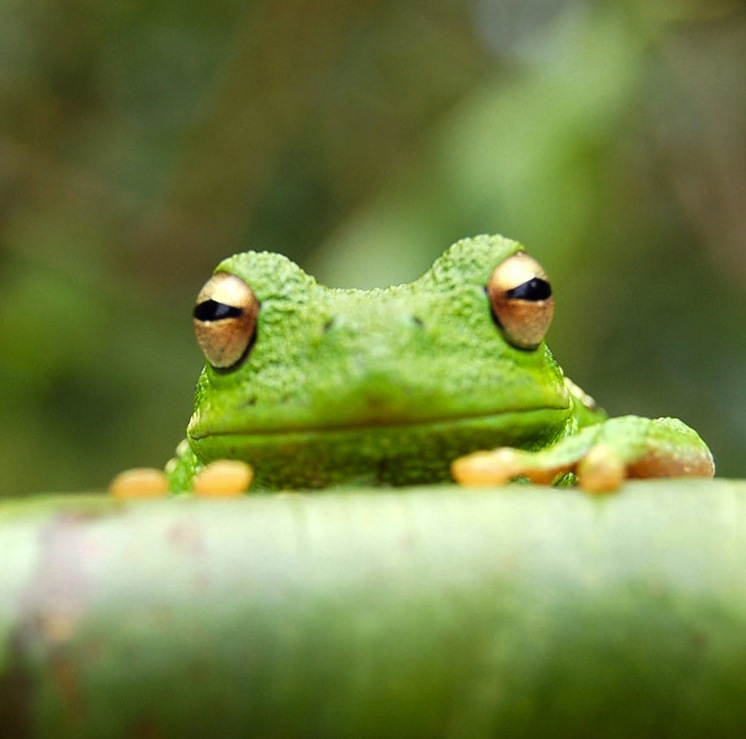
\includegraphics[width=8in]{frog.jpg}
            \end{block}
      \end{column}
      \begin{column}{.3\linewidth}
        	\begin{block}{Introduction}
          		\begin{itemize}
          			\item some items and $\alpha=\gamma, \sum_{i}$
          			\item some items
          			\item some items
          			\item some items
          		\end{itemize}
          		$$\alpha=\gamma, \sum_{i}$$
        	\end{block}
			\vfill
        	\begin{block}{Introduction}
          		\begin{itemize}
          			\item some items
          			\item some items
          			\item some items
          			\item some items
          		\end{itemize}
        	\end{block}
			\vfill
        	\begin{block}{Conclusion}
          		\begin{itemize}
          			\item some items and $\alpha=\gamma, \sum_{i}$
          			\item some items
          			\item some items
          			\item some items
          		\end{itemize}
          		$$\alpha=\gamma, \sum_{i}$$
        	\end{block}
      \end{column}
    \end{columns}
  \end{frame}
\end{document}


%%%%%%%%%%%%%%%%%%%%%%%%%%%%%%%%%%%%%%%%%%%%%%%%%%%%%%%%%%%%%%%%%%%%%%%%%%%%%%%%%%%%%%%%%%%%%%%%%%%%
%%% Local Variables: 
%%% mode: latex
%%% TeX-PDF-mode: t